\renewcommand{\arraystretch}{1.5}
\begin{tabular}{ c | c | c }
\begin{tikzpicture}[scale=0.4]
  \coordinate (a) at (2,3.464);
  \coordinate (b) at (6.5,5);
  \coordinate (c) at (0.3,0.3);
  \coordinate (d) at (4,0);

  \draw[black,fill] (a) circle [radius=0.1cm] ;
  \draw[black,fill] (b) circle [radius=0.1cm] ;
  \draw[black,fill] (c) circle [radius=0.1cm] ;
  \draw[black,fill] (d) circle [radius=0.1cm] ;
  \draw[white] (a) circle [radius=4.2cm] ;
  \draw[white] (b) circle [radius=4.2cm] ;
  \draw[white] (c) circle [radius=4.2cm] ;
  \draw[white] (d) circle [radius=4.2cm] ;
\end{tikzpicture} &
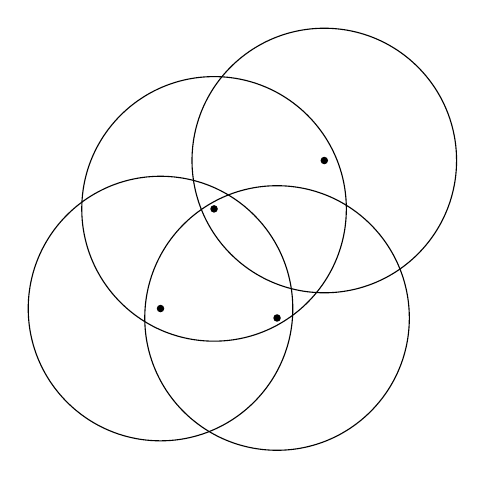
\begin{tikzpicture}[scale=0.4]
  \coordinate (a) at (2,3.464);
  \coordinate (b) at (5.5,5);
  \coordinate (c) at (0.3,0.3);
  \coordinate (d) at (4,0);

  \draw[black,fill] (a) circle [radius=0.1cm] ;
  \draw[black,fill] (b) circle [radius=0.1cm] ;
  \draw[black,fill] (c) circle [radius=0.1cm] ;
  \draw[black,fill] (d) circle [radius=0.1cm] ;
  \draw[black] (a) circle [radius=4.2cm] ;
  \draw[black] (b) circle [radius=4.2cm] ;
  \draw[black] (c) circle [radius=4.2cm] ;
  \draw[black] (d) circle [radius=4.2cm] ;
\end{tikzpicture} &
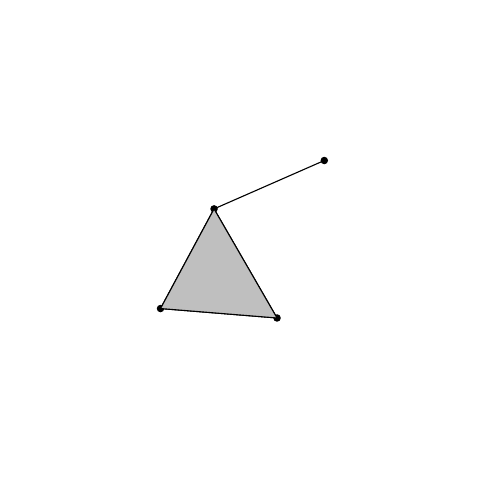
\begin{tikzpicture}[scale=0.4]
  \coordinate (a) at (2,3.464);
  \coordinate (b) at (5.5,5);
  \coordinate (c) at (0.3,0.3);
  \coordinate (d) at (4,0);
  
  \draw[black,fill] (a) circle [radius=0.1cm] ;
  \draw[black,fill] (b) circle [radius=0.1cm] ;
  \draw[black,fill] (c) circle [radius=0.1cm] ;
  \draw[black,fill] (d) circle [radius=0.1cm] ;
    \draw[white] (a) circle [radius=4.2cm] ;
  \draw[white] (b) circle [radius=4.2cm] ;
  \draw[white] (c) circle [radius=4.2cm] ;
  \draw[white] (d) circle [radius=4.2cm] ;
  \draw (c) -- (a) -- (d) -- cycle;
  \draw (b) -- (a);
  \draw[fill=gray!50] (c) -- (a) -- (d) -- cycle;
\end{tikzpicture}
\end{tabular}